%\documentclass[fleqn]{book}
\documentclass[11pt]{amsbook}

\usepackage[turkish]{babel}

%\usepackage{../HBSuerDemir}	% ------------------------
\usepackage{../Ceyhun}	% ------------------------
\usepackage{../amsTurkish}


\begin{document}
% ++++++++++++++++++++++++++++++++++++++
\hPage{089}
% ++++++++++++++++++++++++++++++++++++++

\begin{theorem}
\begin{proof}\footnote{Proof of theorem continues from the previous page of the previous page.}
	\[
		1 \leq k_{1} \leq q/2
	\]
varsayımından dolayı da çizgede kertesi $k_{1}$ den büyük olmayan, $k_{1}$ den az düğüm vardır. Bu çelişki, $Ç$ nin Harnilton çizgesi olması ile ortadan kalkabilir.
\end{proof}
\end{theorem}


Posa teoreminin yalnız bir yeter koşul olduğu ve gerek koşul olamayacağı hemen gösterilebilir. Örneğin, Şekil 2.6.1 deki çizgeler, Harnilton çizgesi olmalarına karşın, Posa Teoremini sağlamamaktadır. Örneğin \reffig{fig:PosaTheoremNotHamiltons}'deki

\begin{figure}[htb]
	\centering
	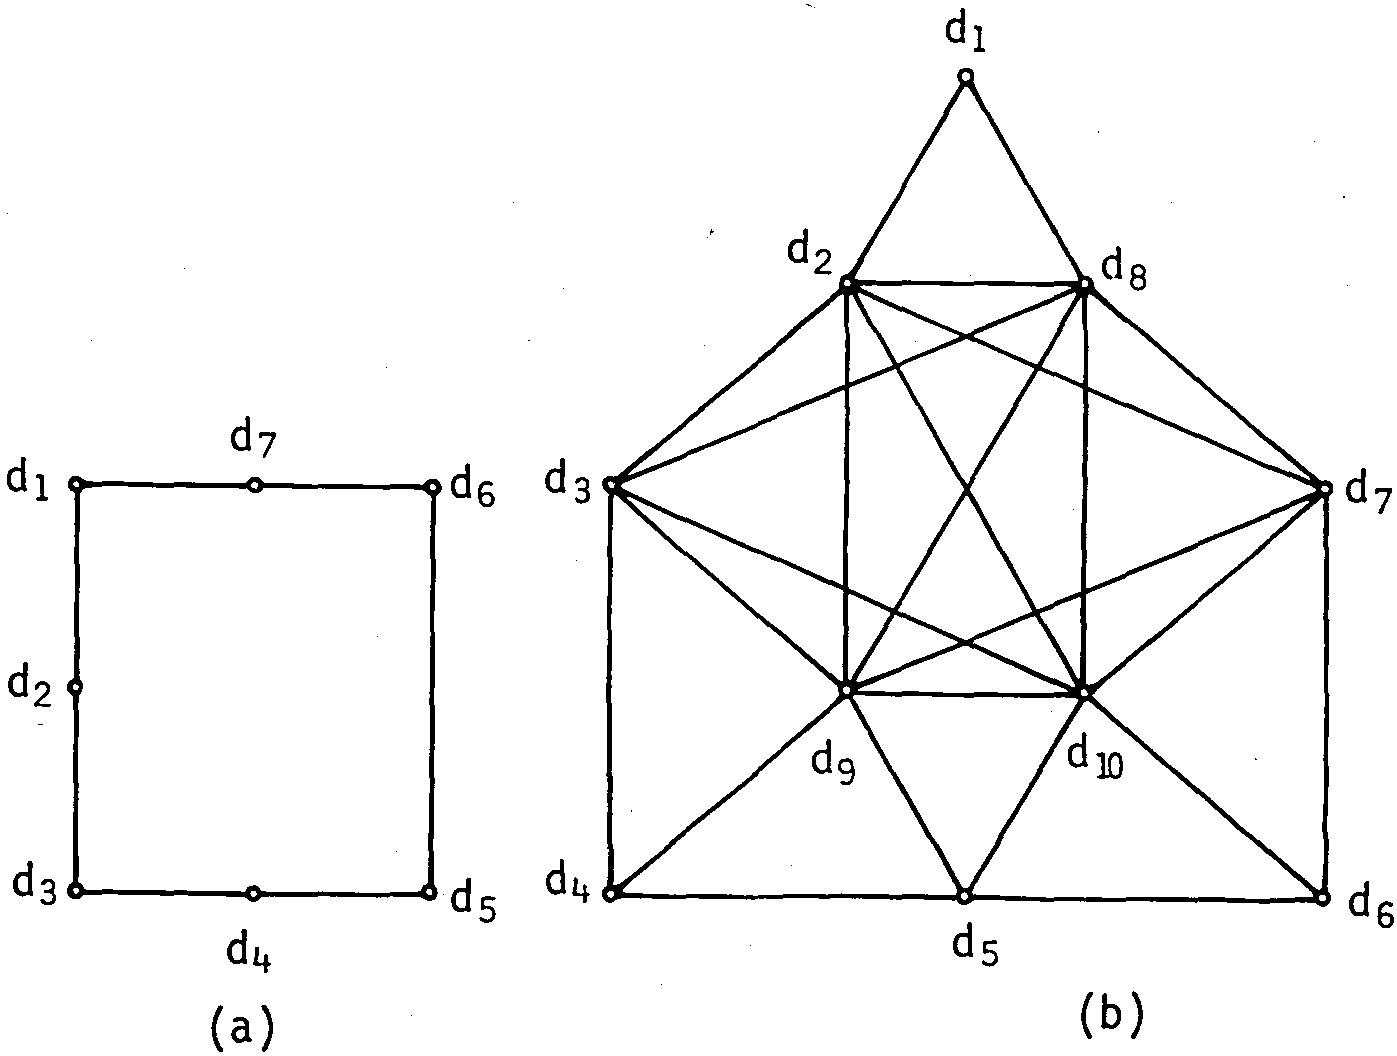
\includegraphics[width=0.45\textwidth]{images/ceyhun-089-fig01.png}
	\caption{Posa Teoremının yeter koşulunu sağlamayan Hamilton çizgeleri.}
	\label{fig:PosaTheoremNotHamiltons}
\end{figure}

\end{document}